\bibliographystyle{babplain-fl}

\chapter{Algoritmos discretos}
\label{cha:discrete-algorithms}

  Nos interesan algoritmos que operan con objetos \emph{discretos}
  (a diferencia de los objetos continuos que hemos discutido hasta acá).
  Nos interesa determinar cuántos recursos
  se requieren para resolver un problema
  (cotas inferiores),
  inventar buenos algoritmos,
  evaluar el rendimiento de los algoritmos para compararlos entre sí
  y para compararlos con cotas teóricas.
  Hay dos maneras en que se organiza la enorme cantidad de material relevante:
  una es dar un catálogo de problemas ordenados por área
  y proponer algoritmos para ellos
  (es fundamentalmente lo que hace el clásico texto de Cormen y otros~%
     \cite{cormen09:_CLRS},
   es la organización del texto de Knuth~%
     \cite{knuth97:_fundam_algor,
           knuth97:_semin_algor,
           knuth98:_sortin_searc,
           knuth11:_combin_alg_1})
  o centrarse en técnicas de diseño y análisis,
  usando problemas en distintas áreas como ilustración
  (como lo hacen Sedgewick y Wayne~%
     \cite{sedgewick11:_algorithms},
   Skiena~%
     \cite{skiena08:_algor_desig_manual}
   y Erickson~%
     \cite{erickson19:_algorithms})
  otros autores combinan ambas formas de abordarlo
  (es el caso de Goodrich y Tamassia~%
     \cite{goodrich01:_algorithm_design}).
  El presente texto se concentra en técnicas de diseño de algoritmos.

  Cuidado,
  mucho del \textquote{análisis tradicional}
  (su indiscutible máximo exponente es Donald Knuth)
  supone que la memoria es rápida
  y acceso a ella es básicamente uniforme.
  La realidad actual
  (desde hace unos 40 años o así)
  es muy diferente,
  como demuestra Kamp~%
    \cite{kamp10:_doing_it_wrong}.
  Si se manejan enormes cantidades de datos,
  la organización de las estructuras de datos puede ser crítica.
  Asimismo,
  el análisis tradicionalmente se concentra en el caso de único procesador,
  máquinas actuales tienen varios de ellos y usarlos efectivamente
  es un tema importante.
  Tarjetas de video actuales son muchísimos procesadores,
  a ser usados en forma especializada
  (básicamente efectuar la misma operación en paralelo sobre datos distintos),
  aprovechar esas facilidades presenta desafíos interesantes.

  Para estimar el tiempo de ejecución de un algoritmo,
  podemos determinar cuántas veces se ejecuta cada instrucción
  (esto generalmente depende de la construcción exacta de los datos,
   con lo que resultan relevantes estadísticas de los datos de entrada,
   que lleva a estadísticas de los números de veces que se ejecuta),
  sabiendo cuánto se demora cada instrucción
  podemos determinar tiempos de ejecución.
  Pero esto significa partir esencialmente con el programa completo,
  ya sea en lenguaje de máquina
  (como ejemplifica Knuth~%
     \cite{knuth97:_fundam_algor, knuth97:_semin_algor,knuth98:_sortin_searc})
  o medir tiempos de ejecución promedio de operaciones básicas del lenguaje,
  como muestra Bentley~%
    \cite{bentley99:_programming_pearls}
  para C
  (pero hay que considerar que compiladores modernos
   efectúan extensas reorganizaciones del código,
   con lo que esto puede dar resultados engañosos).
  Técnicas similares pueden aplicarse para espacio de memoria.
  Nuevamente,
  Bentley~%
    \cite{bentley99:_programming_pearls}
  da código para medir el costo de estructuras en C.

  Estimaciones más sencillas se obtienen definiendo operaciones clave,
  tales que por cada operación clave hay un número acotado de otras operaciones
  (generalmente operaciones centrales o especialmente costosas).
  Contabilizar el número de operaciones clave es menos trabajo,
  muchas veces puede hacerse
  contando solo con una descripción general del algoritmo,
  no un programa detallado.
  Claramente esto nos dará solo cotas de tiempo asintóticas.

  Nos interesan algoritmos eficientes,
  específicamente en tiempo.
  Esto significa tener una medida del tiempo requerido
  para resolver el problema entre manos,
  típicamente medido en término de operaciones clave como descritas antes,
  independiente del algoritmo empleado.
  Por otro lado,
  tenemos algún algoritmo concreto y su análisis.
  En el caso ideal,
  los costos mínimos ideales y del algoritmo propuesto son iguales;
  generalmente serán diferentes,
  e interesa afinar el modelo teórico,
  hallar un algoritmo mejor,
  o ambos.
  Hay que tener cuidado,
  las cotas asintóticas valen cuando el tamaño del problema es muy grande,
  lo que puede significar tamaños fuera del alcance práctico,
  y esconden constantes de proporcionalidad,
  que pueden ser muy grandes.
  El análisis teórico debe refinarse y contrastarse con mediciones
  para situaciones de gran importancia.

  Para mostrar algo de los problemas y técnicas,
  ilustrando el tipo de resultados que buscamos,
  exploraremos un par de problemas muy sencillos:
  dado un arreglo no ordenado de \(n\) enteros diferentes,
  hallar los dos mayores
  y encontrar el menor y el mayor elemento.
  La discusión siguiente se adapta de~%
    \cite{OpenDSA16:_senior_algorithms}.

\section{Hallar el máximo de un arreglo}
\label{sec:max-array}

  Un problema simple es hallar el máximo elemento de un arreglo.
  Es claro que podemos obtener el máximo con \(n - 1\) comparaciones,
  y no puede hacerse mejor
  (con menos de \(n - 1\) comparaciones
   habrá un elemento que no se compara con ningún otro,
   no tenemos garantía de tener el mayor).
  Este razonamiento es correcto,
  pero informal.
  \begin{proposition}
    Para identificar el máximo de \(n\) elementos
    debemos efectuar al menos \(n - 1\) comparaciones.
  \end{proposition}
  \begin{proof}
    Cada vez que se comparan dos elementos,
    uno resulta perdedor
    (es menor que el otro).
    Como cada comparación produce (a lo más) un (nuevo) perdedor,
    y debemos identificar \(n - 1\) perdedores,
    debemos hacer al menos \(n - 1\) comparaciones.
  \end{proof}
  Una demostración alternativa,
  cuya maquinaria nos servirá
  para construir un buen algoritmo más adelante,
  usa el concepto de \emph{poset}
  (de \emph{\foreignlanguage{english}{partially ordered set}},
   conjunto parcialmente ordenado;
   un conjunto con un \emph{orden parcial},
   una relación reflexiva,
   antisimétrica y transitiva).
  En el orden parcial \(\le\) sobre \(\mathscr{U}\)
  dos elementos pueden ser comparables
  (es \(a \le b\) o \(b \le a\))
  o no.
  Por ejemplo,
  dado un conjunto \(\mathscr{A}\),
  la relación subconjunto define un orden parcial sobre \(2^{\mathscr{A}}\);
  no todos los subconjuntos de \(\mathscr{A}\) son comparables.
  El orden parcial puede describirse como un DAG:
  hay un arco de \(a\) a \(b\) si \(a \le b\),
  al ser una relación transitiva no pueden haber ciclos.
  Podemos considerar que nuestro algoritmo va agregando arcos
  según efectúa comparaciones
  (en el fondo,
   construimos el DAG de las relaciones conocidas entre elementos
   hasta explorar lo suficiente para determinar el máximo).
  \begin{proof}
    Iniciamos el algoritmo con \(n\) DAGs de un único vértice
    (no conocemos nada),
    y debemos construir un DAG que contiene todos los elementos
    (y nos permite identificar el máximo).
    El mínimo número de arcos para conectar los \(n\) vértices es \(n - 1\).
  \end{proof}
  El listado~\ref{lst:maximo-a} da el algoritmo obvio.
  \lstinputlisting[float,
                   language=C,
                   firstline = 6,
                   xleftmargin=3em, numbers=left,
                   caption={Hallar el máximo},
                   label=lst:maximo-a]
                   {code/maximum.c}
  Es obvio que efectúa \(n - 1\) comparaciones,
  y nuestro algoritmo es óptimo.

  Es claro que el número de veces
  que se asigna a~\lstinline[language = C]!max!
  es \(O(n)\);
  es claro que el máximo es \(n\)
  (si \lstinline[language = C]!a! viene ordenado de menor a mayor),
  el mínimo es \num{1}
  (si \lstinline[language = C]!a[0]! es el mayor),
  pero interesa el número promedio de veces.
  Calcular el promedio presenta otro conjunto de problemas:
  ¿Cómo vienen distribuidos los datos?
  Un modelo simple
  (¡que en casos importantes deberá verificarse que se cumple!)
  es suponer que los datos son todos distintos
  y que todos los órdenes de los datos de entrada
  son igualmente probables.
  Se asigna a~\lstinline[language = C]!max!
  en la iteración~\lstinline[language = C]!i!
  si y solo si~\lstinline[language = C]!a[i]!
  es el máximo de los primeros~\lstinline[language = C]!i + 1! elementos.
  Suponiendo que el orden es aleatorio,
  la probabilidad de esto es \(1 / i\).
  Sumando,
  el número promedio de asignaciones es:
  \begin{equation*}
    \sum_{0 \le i \le n - 1} \frac{1}{i + 1}
      = \sum_{1 \le i \le n} \frac{1}{i}
      = H_n
  \end{equation*}
  Sabemos que
  (vea por ejemplo el apéndice~\ref{apx:asymptotics}):
  \begin{equation*}
    \ln n \le H_n < \ln n + 1
  \end{equation*}
  Esto muestra también que nuestra intuición suele engañarnos:
  antes de ver este desarrollo
  creía que se asignaba aproximadamente la mitad de las veces.
  O sea,
  calculaba que si se buscaba el máximo de un millón de elementos,
  se harían unas 500~mil comparaciones.
  En promedio son en realidad \(H_{1\,000\,000} = 14,393\)~comparaciones..
  También muestra que puede resultar relevante
  usar diferentes medidas de comportamiento,
  en este caso número de comparaciones o de asignaciones.

\section{Dos mayores elementos}
\label{sec:dos-mayores}

  Habiendo ubicado el mayor,
  podemos identificar al segundo con \(n - 2\) comparaciones adicionales,
  para un total de \(2 n - 3\).
  Pero esto no considera la información
  que entregan las comparaciones para obtener el máximo.
  Note que los candidatos a segundo lugar
  son los que perdieron al comparar con el máximo,
  queremos el máximo de estos.
  Obtenemos el máximo de información
  al comparar dos elementos que sabemos mayores que el mismo número de valores.
  Esto lleva a comparar pares,
  comparar los máximos de los pares,
  y así sucesivamente.
  Consideremos \emph{árboles binomiales},
  el árbol binomial \(B_0\) es un único vértice,
  y \(B_k\) se construye uniendo dos árboles binomiales \(B_{k - 1}\),
  haciendo que la raíz de uno sea hijo de la raíz del otro
  (ver la figura~\ref{fig:binomial-trees-a}).
  El árbol \(B_k\) tiene \(2^k\) vértices,
  la raíz de \(B_k\) tiene \(k\)~hijos.
  \begin{figure}[ht]
    \centering
    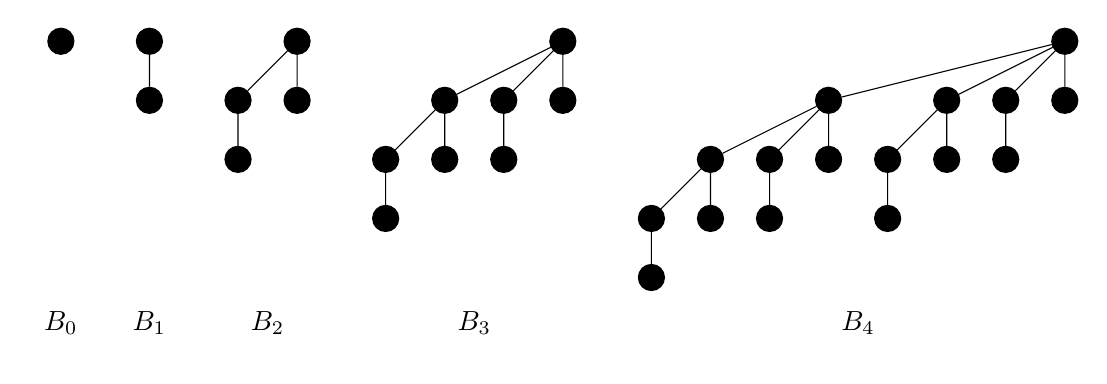
\begin{tikzpicture}[every node/.style = {shape = circle, fill, draw},
                        scale = 0.75]
      \node (a0) at (0, 4) {};
      \node [draw = none, fill = none, below] at (0, -0.2) {\(B_0\)};

      \node (b0) at (1.5, 3) {};
      \node (b1) at (1.5, 4) {};
      \draw (b0) -- (b1);
      \node [draw = none, fill = none, below] at (1.5, -0.2) {\(B_1\)};

      \node (c0) at (3.0, 2) {};
      \node (c1) at (3.0, 3) {};
      \node (c2) at (4.0, 3) {};
      \node (c3) at (4.0, 4) {};
      \draw (c0) -- (c1)
            (c1) -- (c3)
            (c2) -- (c3);
      \node [draw = none, fill = none, below] at (3.5, -0.2) {\(B_2\)};

      \node (d0) at (5.5, 1) {};
      \node (d1) at (5.5, 2) {};
      \node (d2) at (6.5, 2) {};
      \node (d3) at (6.5, 3) {};
      \node (d4) at (7.5, 2) {};
      \node (d5) at (7.5, 3) {};
      \node (d6) at (8.5, 3) {};
      \node (d7) at (8.5, 4) {};
      \draw (d0) -- (d1)
            (d1) -- (d3)
            (d2) -- (d3)
            (d4) -- (d5)
            (d6) -- (d7)
            (d3) -- (d7)
            (d5) -- (d7);
      \node [draw = none, fill = none, below] at (7, -0.2) {\(B_3\)};

      \node (e0)  at (10, 0) {};
      \node (e1)  at (10, 1) {};
      \node (e2)  at (11, 1) {};
      \node (e3)  at (11, 2) {};
      \node (e4)  at (12, 1) {};
      \node (e5)  at (12, 2) {};
      \node (e6)  at (13, 2) {};
      \node (e7)  at (13, 3) {};
      \node (e8)  at (14, 1) {};
      \node (e9)  at (14, 2) {};
      \node (e10) at (15, 2) {};
      \node (e11) at (15, 3) {};
      \node (e12) at (16, 2) {};
      \node (e13) at (16, 3) {};
      \node (e14) at (17, 3) {};
      \node (e15) at (17, 4) {};
      \draw (e0) -- (e1)
            (e1) -- (e3)
            (e2) -- (e3)
            (e4) -- (e5)
            (e6) -- (e7)
            (e3) -- (e7)
            (e5) -- (e7)
            (e8) -- (e9)
            (e9) -- (e11)
            (e10) -- (e11)
            (e12) -- (e13)
            (e13) -- (e15)
            (e14) -- (e15)
            (e11) -- (e15)
            (e7) -- (e15);
      \node [draw = none, fill = none, below] at (13.5, -0.2) {\(B_4\)};
    \end{tikzpicture}
    \caption{Árboles binomiales}
    \label{fig:binomial-trees-a}
  \end{figure}
  Nuestra estrategia es entonces comparar pares,
  comparar los ganadores de los pares,
  y continuar comparando solo ganadores;
  estamos construyendo y uniendo
  árboles binomiales.
  El árbol final es parte de un árbol binomial,
  en determinar el máximo efectuamos \(n - 1\) comparaciones,
  si la raíz
  (el máximo)
  tiene \(k\)~descendientes,
  debemos obtener el máximo de estos para determinar el segundo,
  con un costo de \(k - 1\)~comparaciones adicionales.
  El total de comparaciones es \(n + k - 2\).
  Pero el árbol tiene entre \(2^{k - 1}\) y \(2^k\) vértices en total,
  con lo que \(k = \lceil \log_2 n \rceil\),
  con lo que el número de comparaciones es \(n + \lceil \log_2 n \rceil - 2\).

  Esto claramente es mucho mejor que la idea original
  (pero más complejo).
  ¿Es el mejor posible?
  Una técnica para demostrar que un algoritmo es óptimo
  es imaginar un adversario,
  que en cada paso responde lo peor posible
  (consistente con sus respuestas anteriores,
   claro está).
  Nuevamente consideramos el modelo de construir un DAG
  que nos entregue el máximo y el segundo mayor elemento,
  sin restringirnos ahora a un árbol binomial.
  Antes de ir a la demostración misma,
  observamos que los primeros \(n - 1\)~elementos
  tienen que haber perdido al menos una comparación,
  se requieren al menos \(n - 1\) comparaciones.
  Adicionalmente,
  al menos \(k - 1\)~elementos perdieron contra el segundo mayor
  (los \(k\) perdedores de las comparaciones con el máximo),
  haciendo un total de \(n + k - 2\) comparaciones.
  La pregunta entonces es,
  ¿qué tan pequeño podemos hacer \(k\)?
  Llamemos \emph{poder} de~\lstinline[language = C]!a[i]!
  al número de elementos que sabemos son menores a él.
  Si~\lstinline[language = C]!a[i]! tiene poder~\(a\)
  y~\lstinline[language = C]!a[j]! tiene poder~\(b\),
  el ganador de la comparación entre ellos tiene poder~\(a + b + 1\).
  Nuestro algoritmo conoce los poderes (actuales) de cada elemento,
  y debe decidir cuáles de ellos comparar a continuación.
  El adversario decide el resultado de la comparación,
  y busca entregar la mínima información con el.
  Esto corresponde a minimizar el aumento de poder de cualquier elemento,
  o sea siempre dar por ganador al elemento con mayor poder.
  Esto es construir el peor caso de datos al algoritmo,
  no es injusto.

  Queremos minimizar el efecto del peor caso,
  esto es maximizar el aumento mínimo de poder
  balanceando los poderes de los contendores.
  El mejor caso se da si el poder del ganador se duplica,
  vale decir,
  si el poder de ambos es el mismo.
  Como los poderes comienzan en cero,
  el ganador tiene que efectuar al menos \(k\)~comparaciones,
  donde \(2^{k - 1} < n \le 2^k\).
  O sea,
  \(k = \lceil \log_2 n \rceil\),
  nuestro algoritmo es óptimo.

\section{Máximo y mínimo}
\label{sec:maximo-minimo}

  Nuestro siguiente problema,
  hallar el máximo y el mínimo,
  es superficialmente similar al anterior,
  pero requiere métodos de análisis diferentes.
  Nuevamente consideremos solo el número de comparaciones.
  Una primera idea es recorrer el arreglo,
  recordando el máximo y el mínimo vistos hasta el momento,
  vea el listado~\ref{lst:max-min}.
  \lstinputlisting[float,
                   language=C,
                   firstline = 8,
                   xleftmargin=3em, numbers=left,
                   caption={Hallar el máximo y el mínimo},
                   label=lst:max-min]
                   {code/max-min.c}
  Es claro que esto es el doble de trabajo que solo obtener el máximo,
  listado~\ref{lst:maximo-a}.
  No estamos aprovechando bien el trabajo hecho al comparar,
  analicemos alternativas.

  Una opción es dividir el conjunto en dos,
  hallar (recursivamente) máximo y mínimo en ambas partes,
  y comparar los máximos y los mínimos de las partes.
  El listado~\ref{lst:max-min-d&c} da detalles.
  \lstinputlisting[float,
                   language=C,
                   firstline = 8,
                   xleftmargin=3em, numbers=left,
                   caption={Hallar el máximo y el mínimo, dividiendo en dos},
                   label=lst:max-min-d&c]
                   {code/max-min-dc.c}
  Si dividimos lo más equitativamente posible,
  el número de comparaciones para \(n\)~elementos,
  \(T(n)\),
  cumple:
  \begin{equation}
    \label{eq:max-min-recursion-1}
    T(n)
      = \begin{cases}
          0							& n = 1	  \\
          1							& n = 2	  \\
          T(\lfloor n / 2 \rfloor) + T(\lceil n / 2 \rceil) + 2 & n \ge 2
        \end{cases}
  \end{equation}
  Esta recurrencia tiene una solución complicada.
  Pero vemos directamente que si \(n = 2^k\) o \(n = 2^k \pm 1\),
  la solución es \(T(n) = 3 n / 2 - 2\);
  cuando \(n = 3 \cdot 2^k\) es \(T(n) = 5 n / 3 - 2\).

  En realidad,
  nada obliga a dividir aproximadamente en dos partes iguales,
  la recurrencia real debiera ser:
  \begin{equation}
    \label{eq:max-min-recursion-2}
    T(n)
      = \begin{cases}
          0							& n = 1	  \\
          1							& n = 2	  \\
          \min_{1 \le k < n} \{ T(k) + T(n - k) \} + 2		& n \ge 2
        \end{cases}
  \end{equation}
  Experimentando con esta nueva versión,
  vemos que siempre obtenemos el mínimo con \(k = 2\),
  lo que lleva a la recurrencia:
  \begin{equation}
    \label{eq:max-min-recursion}
    T(n)
      = \begin{cases}
          0			& n = 1	  \\
          1			& n = 2	  \\
          T(n - 2) + 3		& n \ge 2
        \end{cases}
  \end{equation}
  La solución es \(T(n) = \lceil 3 n / 2 \rceil - 2\)
  (resuelva pares e impares por separado,
   combine las soluciones).
  El código sugerido por esta recurrencia
  (traducido de recursión a iteración)
  es el dado por el listado~\ref{lst:max-min-opt}.
  \lstinputlisting[float,
                   language=C,
                   firstline = 8,
                   xleftmargin=3em, numbers=left,
                   caption={Hallar el máximo y el mínimo, versión mejorada},
                   label=lst:max-min-opt]
                   {code/max-min-opt.c}
  La pregunta obvia es si esto es óptimo.
  Para demostrarlo,
  agregamos otra herramienta a nuestro arsenal,
  usar un espacio de estados.

  En cada momento de la ejecución de cualquier algoritmo
  podemos representar lo que \textquote{sabe}
  registrando el número de \emph{ganadores} \(W\),
  elementos que han sido comparados con otros y nunca han perdido;
  \emph{perdedores} \(L\),
  elementos que han sido comparados con otros y nunca han ganado;
  elementos \emph{no comparados} \(U\);
  y elementos \emph{medios} \(M\),
  han sido comparados y han ganado y perdido.
  La situación inicial es \((U, W, L, M) = (n, 0, 0, 0)\),
  la situación final es \((0, 1, 1, n - 2)\).
  Con cuatro tipos de elementos,
  hay diez tipos de comparaciones posibles.
  Comparar \(M\) con otros no tiene sentido,
  puede cambiar a lo más la clasificación del otro elemento.
  Quedan seis comparaciones de interés,
  cuyos efectos sobre el estado \((U, W, L, M) = (i, j, k, l)\)
  resume el cuadro~\ref{tab:comparison-efect}.
  \begin{table}[ht]
    \centering
    \begin{tabular}{>{\(}c<{\)}|*{4}{>{\(}l<{\)}}}
      & \multicolumn{1}{c}{\boldmath\(U\)\unboldmath} &
        \multicolumn{1}{c}{\boldmath\(W\)\unboldmath} &
        \multicolumn{1}{c}{\boldmath\(L\)\unboldmath} &
        \multicolumn{1}{c}{\boldmath\(M\)\unboldmath} \\
      \hline
      U \colon U & i - 2 & j + 1 & k + 1 & l	 \\
      \hline
      W \colon W & i	 & j - 1 & k	 & l + 1 \\
      \hline
      L \colon L & i	 & j	 & k - 1 & l + 1 \\
      \hline
      \multirow{2}{*}{\(L \colon U\)}
                & i - 1 & j + 1 & k	 & l	 \\
                & i - 1 & j	 & k	 & l + 1 \\
      \hline
      \multirow{2}{*}{\(W \colon U\)}
                 & i - 1 & j	 & k + 1 & l	 \\
                 & i - 1 & j	 & k	 & l + 1 \\
      \hline
      \multirow{2}{*}{\(W \colon L\)}
                 & i	 & j	 & k	 & l	 \\
                 & i	 & j - 1 & k - 1 & l + 2 \\
      \hline
    \end{tabular}
    \caption{Comparaciones y sus efectos}
    \label{tab:comparison-efect}
  \end{table}
  Consideremos nuevamente un adversario,
  que dicta los resultados de las comparaciones
  de manera que el algoritmo trabaje lo más posible,
  vale decir,
  elige la alternativa que menos acerca al resultado deseado.
  Por ejemplo,
  comparar un ganador con un perdedor en el peor caso no da información nueva
  (el perdedor pierde y el ganador gana).
  Eliminado las alternativas que en el peor caso no aportan información nueva,
  quedan las del cuadro~\ref{tab:comparison-efect-select}.
  \begin{table}[ht]
    \centering
    \begin{tabular}{>{\(}c<{\)}|*{4}{>{\(}l<{\)}}}
      & \multicolumn{1}{c}{\boldmath\(U\)\unboldmath} &
        \multicolumn{1}{c}{\boldmath\(W\)\unboldmath} &
        \multicolumn{1}{c}{\boldmath\(L\)\unboldmath} &
        \multicolumn{1}{c}{\boldmath\(M\)\unboldmath} \\
      \hline
      U \colon U & i - 2 & j + 1 & k + 1 & l	 \\
      L \colon U & i - 1 & j + 1 & k	 & l	 \\
      W \colon U & i - 1 & j	 & k + 1 & l	 \\
      \hline
      W \colon W & i	 & j - 1 & k	 & l + 1 \\
      L \colon L & i	 & j	 & k - 1 & l + 1 \\
      \hline
    \end{tabular}
    \caption{Comparaciones interesantes y sus efectos}
    \label{tab:comparison-efect-select}
  \end{table}
  Solo las últimas dos transiciones
  del cuadro~\ref{tab:comparison-efect-select}
  aumentan el número de \(M\),
  debe haber un mínimo de \(n - 2\) de estas.
  El número de elementos sin comparar debe llegar a cero,
  y la primera transición es la más eficiente en esto,
  se requieren \(\lfloor n / 2 \rfloor\) de estas,
  junto a una comparación \(L \colon U\) o \(W \colon U\)
  si \(n\) es impar,
  para hacer cero \(U\),
  o sea \(\rceil n / 2 \lceil\)~comparaciones
  En total,
  se necesitan al menos \(n - 2 + \lceil n / 2 \rceil\)~comparaciones.
  Nuestro algoritmo es óptimo.

\section*{Ejercicios}
\label{sec:exercises-07-pre-previa}

  \begin{enumerate}
  \item
    Demuestre que \(k = 2\) siempre da un mínimo
    en la recurrencia~\eqref{eq:max-min-recursion-2}.
  \item
    Escriba un programa que halle el máximo y segundo elemento de un arreglo
    usando el algoritmo óptimo esbozado en el texto.
  \item
    Evalúe el número promedio de asignaciones de elementos en el programa
    del listado~\ref{lst:max-min}.
    Es claro que la segunda comparación fallará si tiene éxito la primera,
    evalúe el efecto de considerar esto.
  \item
    Considere el problema de hallar los tres mayores elementos.
    ¿Cuántas comparaciones requiere?
  \end{enumerate}

\bibliography{../referencias}

%%% Local Variables:
%%% mode: latex
%%% TeX-master: "../INF-221_notas"
%%% ispell-local-dictionary: "spanish"
%%% End:

% LocalWords:  poset english partially ordered set antisimétrica DAG
% LocalWords:  DAGs contendores eq max min recursion
